% This is now Chapter 3
This section outlines the research design, data collection methods, and analytical techniques employed in this comparative study of teacher evaluation approaches.

\subsection{Research Design and Approach}
This study employs a mixed-methods comparative design to evaluate traditional student feedback and multimodal evaluation systems. The research follows a parallel convergent approach where both evaluation methods are applied simultaneously to the same teaching instances, allowing for direct comparison while minimizing contextual variations.
The study will be conducted in a real-world classroom setting, focusing on higher education institutions. The multimodal evaluation system will be implemented in a controlled environment, ensuring that both student feedback and multimodal data are collected under similar conditions. This design allows for a comprehensive analysis of the strengths and weaknesses of each evaluation method.
The research will utilize a combination of quantitative and qualitative data collection methods, including standardized surveys, audio-visual recordings, and discourse analysis \cite{dmello2012multimodal, ochoa2016multimodal}. The quantitative data will be analyzed using statistical techniques to identify correlations and patterns, while qualitative data will undergo thematic analysis to extract meaningful insights.
The study will also incorporate a longitudinal component, allowing for the examination of changes in teaching effectiveness over time. By collecting data at multiple points throughout the semester, the research aims to capture the dynamic nature of teaching and learning processes.

\begin{table}[H]
    \normalsize
    \centering
    \caption{ Participant Distribution Across Disciplines and Experience Levels}
    \label{tab:participants}
    \begin{tabular}{lccc}
        \toprule
        \textbf{Discipline} & \textbf{Novice} & \textbf{Experienced} & \textbf{Expert} \\
        \midrule
        STEM & 4 & 4 & 2 \\
        Humanities & 4 & 4 & 2 \\
        Social Sciences & 4 & 4 & 2 \\
        \bottomrule
    \end{tabular}
\end{table}

\subsection{Participants and Sampling}
The study will employ purposive sampling to select 30 instructors from diverse academic disciplines. The inclusion criteria prioritize representativeness across teaching experience (novice to expert), course level (undergraduate and graduate), and subject area (STEM, humanities, and social sciences). Each instructor will be evaluated during 3 different teaching sessions, generating a total of 90 distinct teaching instances for analysis.


Student evaluators will include all enrolled students in the selected course sections, with an estimated total of 1,200-1,500 student participants. Demographic information will be collected from both instructors and students to examine potential correlation patterns and biases.

\subsection{Data Collection Methods}

\subsubsection{Student Feedback Instruments}
Traditional evaluation data will be collected using two complementary instruments. First, a standardized quantitative evaluation form using a 5-point Likert scale covering seven dimensions of teaching effectiveness: clarity, organization, engagement, assessment, feedback, accessibility, and overall effectiveness. Second, open-ended qualitative questions eliciting specific comments on teaching strengths, areas for improvement, and notable classroom experiences.

\begin{figure}[ht]
    \centering
    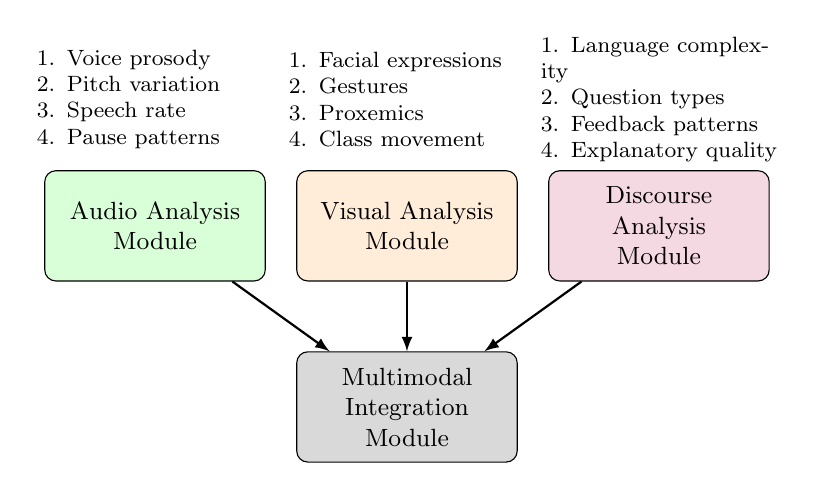
\begin{tikzpicture}[
        module/.style={rectangle, draw, rounded corners, minimum width=2.8cm, minimum height=1.4cm, text width=2.2cm, align=center, font=\small},
        arrow/.style={->, thick, >=latex}
    ]
        % Central component
        \node[module, fill=gray!30] (central) at (0,0) {Multimodal Integration Module};
        
        % Source modules (spaced further apart)
        \node[module, fill=green!15] (audio) at (-3.2,2.3) {Audio Analysis Module};
        \node[module, fill=orange!15] (visual) at (0,2.3) {Visual Analysis Module};
        \node[module, fill=purple!15] (text) at (3.2,2.3) {Discourse Analysis Module};
        
        % Connect modules
        \draw[arrow] (audio) -- (central);
        \draw[arrow] (visual) -- (central);
        \draw[arrow] (text) -- (central);
        
        % Features for each module (moved above and spaced)
        \node[text width=3.0cm, align=left, font=\footnotesize, yshift=0.9cm] at (audio.north) {1. Voice prosody\\2. Pitch variation\\3. Speech rate\\4. Pause patterns};
        \node[text width=3.0cm, align=left, font=\footnotesize, yshift=0.9cm] at (visual.north) {1. Facial expressions\\2. Gestures\\3. Proxemics\\4. Class movement};
        \node[text width=3.0cm, align=left, font=\footnotesize, yshift=0.9cm] at (text.north) {1. Language complexity\\2. Question types\\3. Feedback patterns\\4. Explanatory quality};
    \end{tikzpicture}
    \centering
    \caption{\centering Multimodal system components and feature extraction modules.}
    \label{fig:multimodal_components}
\end{figure}


\subsubsection{Multimodal System Components}
The multimodal evaluation system integrates data from three primary sources, as illustrated in Figure \ref{fig:multimodal_components}. The audio module captures speech dynamics using directional microphones positioned strategically in the classroom, extracting features related to vocal variety, speech clarity, and emotional tone. The visual module employs two wide-angle cameras placed at the front and rear to capture teacher movements, gestures, and interactions with students, while a deep learning-based pose estimation algorithm tracks key behavioral indicators. The discourse module applies natural language processing techniques to analyze transcribed classroom dialogue, identifying patterns of instruction, questioning techniques, and feedback quality. Data collection for both the traditional evaluation and multimodal system occurs simultaneously during the same teaching sessions to ensure valid comparisons.



\begin{enumerate}
    \item \textbf{Audio Module:} Captures speech dynamics using directional microphones positioned strategically in the classroom. The system extracts features related to vocal variety, speech clarity, and emotional tone.
    
    \item \textbf{Visual Module:} Employs two wide-angle cameras (front and rear) to capture teacher movements, gestures, and interactions with students. A deep learning-based pose estimation algorithm tracks key behavioral indicators.
    
    \item \textbf{Discourse Module:} Applies NLP techniques to analyze transcribed classroom dialogue, identifying patterns of instruction, questioning techniques, and feedback quality.
\end{enumerate}

Data collection will occur simultaneously for both evaluation methods during the same teaching sessions to ensure valid comparisons.


\subsection{Data Processing and Feature Extraction}

\subsubsection{Audio Data Processing}
Audio data will be processed to extract the following features:
\begin{itemize}
    \item Prosodic features (pitch, intensity, and speech rate)
    \item Voice quality parameters (jitter, shimmer, and harmonic-to-noise ratio)
    \item Temporal features (speaking time, pause duration, and turn-taking patterns)
    \item Emotion indicators (valence and arousal levels)
\end{itemize}

Audio processing will employ the PRAAT acoustic analysis software with custom scripts for feature extraction, followed by normalization to account for individual voice characteristics.

\subsubsection{Visual Data Analysis}
Visual analysis will focus on extracting behavioral indicators using the following pipeline:

\begin{figure}[t]
    \centering
    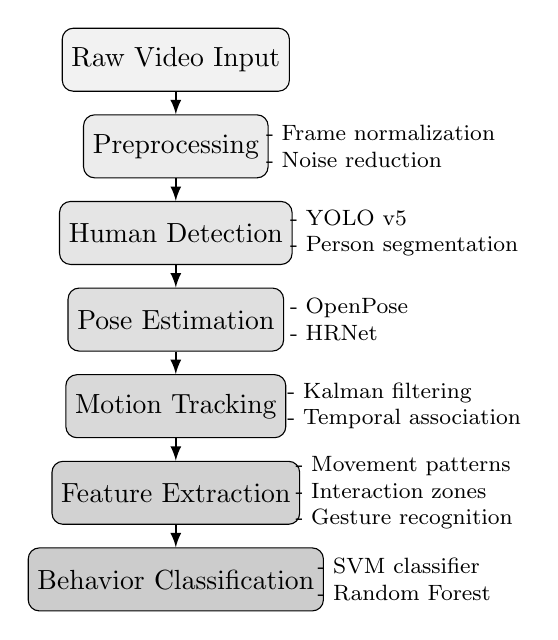
\begin{tikzpicture}[
        stage/.style={rectangle, draw, rounded corners, minimum width=1.8cm, minimum height=0.8cm, align=center, font=\normalsize},
        arrow/.style={->, thick, >=latex}
    ]
        % Processing stages
        \node[stage, fill=gray!10] (input) at (0,0) {Raw Video Input};
        \node[stage, fill=gray!15] (preproc) at (0,-1.1) {Preprocessing};
        \node[stage, fill=gray!20] (detect) at (0,-2.2) {Human Detection};
        \node[stage, fill=gray!25] (pose) at (0,-3.3) {Pose Estimation};
        \node[stage, fill=gray!30] (track) at (0,-4.4) {Motion Tracking};
        \node[stage, fill=gray!35] (extract) at (0,-5.5) {Feature Extraction};
        \node[stage, fill=gray!40] (classify) at (0,-6.6) {Behavior Classification};
        
        % Connect stages
        \draw[arrow] (input) -- (preproc);
        \draw[arrow] (preproc) -- (detect);
        \draw[arrow] (detect) -- (pose);
        \draw[arrow] (pose) -- (track);
        \draw[arrow] (track) -- (extract);
        \draw[arrow] (extract) -- (classify);
        
        % Key techniques
        \node[font=\footnotesize, align=left] at (2.6,-1.1) {- Frame normalization\\- Noise reduction};
        \node[font=\footnotesize, align=left] at (2.9,-2.2) {- YOLO v5\\- Person segmentation};
        \node[font=\footnotesize, align=left] at (2.2,-3.3) {- OpenPose\\- HRNet};
        \node[font=\footnotesize, align=left] at (2.9,-4.4) {- Kalman filtering\\- Temporal association};
        \node[font=\footnotesize, align=left] at (2.9,-5.5) {- Movement patterns\\- Interaction zones\\- Gesture recognition};
        \node[font=\footnotesize, align=left] at (2.9,-6.6) {- SVM classifier\\- Random Forest};
    \end{tikzpicture}
    \caption{ Visual data processing pipeline for teacher behavior analysis.}
    \label{fig:vision_pipeline}
\end{figure}

The system will quantify spatial classroom dynamics, including:
\begin{itemize}
    \item Classroom coverage (percentage of classroom space utilized)
    \item Proximity patterns (time spent in different classroom zones)
    \item Student interaction frequency (number and distribution of individual engagements)
    \item Gesture frequency and type (emphatic, illustrative, and regulatory)
\end{itemize}

\subsubsection{Linguistic and Discourse Analysis}
Classroom dialogue will be transcribed automatically using speech-to-text technology and analyzed for:
\begin{itemize}
    \item Question complexity (based on Bloom's taxonomy)
    \item Wait time after questions
    \item Feedback patterns (evaluative, corrective, or elaborative)
    \item Language complexity (lexical diversity and sentence structure)
    \item Instructional clarity indicators (use of examples, analogies, and summaries)
\end{itemize}

\subsubsection{Student Feedback Processing}
Quantitative feedback will be analyzed using descriptive and inferential statistics, while qualitative comments will undergo thematic analysis using a dual-coding approach to identify emergent patterns. NLP techniques will also be applied to extract sentiment and topical focus from written comments.

\subsection{System architecture}
% This is now Chapter 5

The proposed system is a modular, end-to-end multimodal machine learning pipeline that processes audio, video, and transcript data streams in parallel, fuses their representations, and predicts teaching effectiveness using a unified classifier. This architecture leverages state-of-the-art models and best practices from the HuggingFace ecosystem and the broader machine learning community.

\begin{figure}[H]
    \centering
    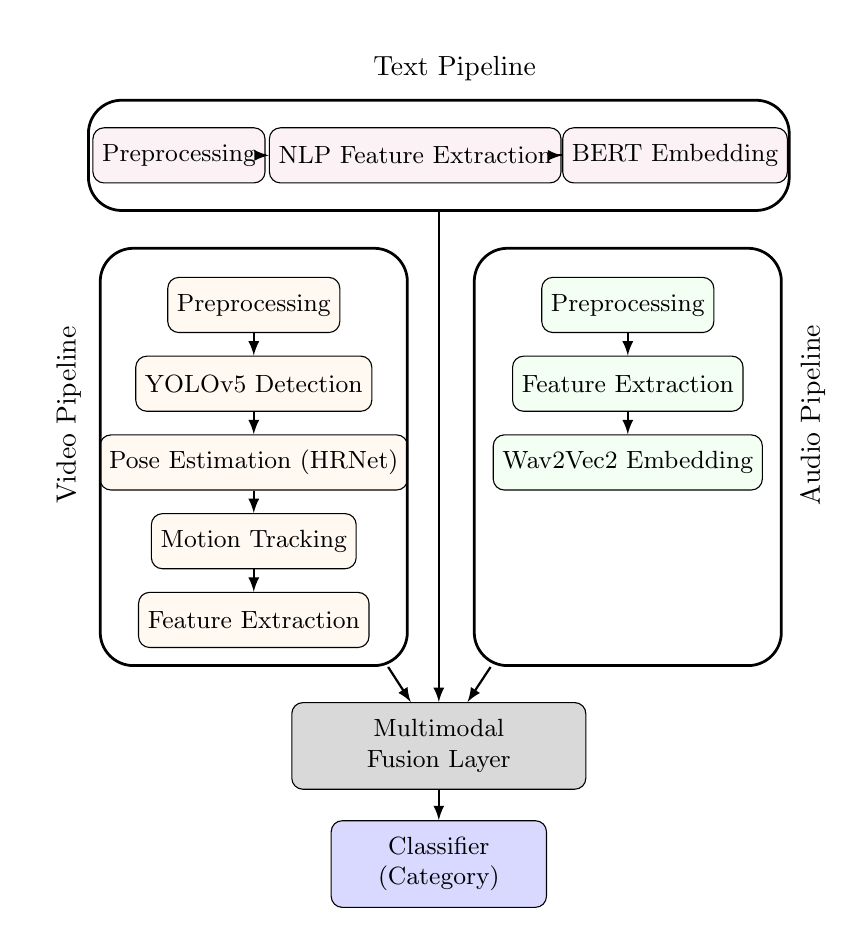
\begin{tikzpicture}[
        module/.style={rectangle, draw, rounded corners, minimum width=2.5cm, minimum height=1.1cm, text width=2.5cm, align=center, font=\small, fill=gray!10},
        arrow/.style={->, thick, >=latex},
        process/.style={rectangle, draw, rounded corners, minimum width=2cm, minimum height=0.7cm, font=\small, fill=white},
        pipelinebox/.style={draw=black, rounded corners=12pt, line width=1pt, minimum width=3.2cm, minimum height=5.3cm}
    ]

        % Text pipeline
        \node[process, fill=purple!5] (t1) at (-6.2,3.3) {Preprocessing};
        \node[process, fill=purple!5] (t2) at (-3.2,3.3) {NLP Feature Extraction};
        \node[process, fill=purple!5] (t3) at (0.1,3.3) {BERT Embedding};
        \node[pipelinebox,rotate=0, minimum width=8.9cm,minimum height=1.4cm, fill=none] (cover3) at (-2.9,3.3) {};
        \node[label, rotate=0, xshift=-2.7cm,yshift=4.4cm] {Text Pipeline};

        % Video pipeline
        \node[process, fill=orange!5] (v1) at (-5.25,1.4) {Preprocessing};
        \node[process, fill=orange!5] (v2) at (-5.25,0.4) {YOLOv5 Detection};
        \node[process, fill=orange!5] (v3) at (-5.25,-0.6) {Pose Estimation (HRNet)};
        \node[process, fill=orange!5] (v4) at (-5.25,-1.6) {Motion Tracking};
        \node[process, fill=orange!5] (v5) at (-5.25,-2.6) {Feature Extraction};
        \node[pipelinebox,minimum width=3.9cm, fill=none] (cover1) at (-5.25,-.53) {};
        \node[label, rotate=90, xshift=0cm,yshift=7.6cm] {Video Pipeline};


        % Audio pipeline
        \node[process, fill=green!5] (a1) at (-0.5,1.4) {Preprocessing};
        \node[process, fill=green!5] (a2) at (-0.5,0.4) {Feature Extraction};
        \node[process, fill=green!5] (a3) at (-0.5,-0.6) {Wav2Vec2 Embedding};
        \node[pipelinebox, minimum width=3.9cm,fill=none] (cover2) at (-0.5,-.53) {};
        \node[label, rotate=90, xshift=0cm,yshift=-1.85cm] {Audio Pipeline};

       

        % Fusion and classifier
        \node[module, fill=gray!30, minimum width=3.5cm, text width=3.5cm] (fusion) at (-2.9,-4.2) {Multimodal Fusion Layer};
        \node[module, fill=blue!15, minimum width=2.5cm, text width=2.5cm] (clf) at (-2.9,-5.7) {Classifier\\(Category)};

        % Arrows for video
        \draw[arrow] (v1) -- (v2);
        \draw[arrow] (v2) -- (v3);
        \draw[arrow] (v3) -- (v4);
        \draw[arrow] (v4) -- (v5);
        \draw[arrow] (cover1) -- (fusion);

        % Arrows for audio
        \draw[arrow] (a1) -- (a2);
        \draw[arrow] (a2) -- (a3);
        \draw[arrow] (cover2) -- (fusion);

        % Arrows for text
        \draw[arrow] (t1) -- (t2);
        \draw[arrow] (t2) -- (t3);
        \draw[arrow] (cover3) -- (fusion);

        % Fusion to classifier
        \draw[arrow] (fusion) -- (clf);

    \end{tikzpicture}
    \centering
    \caption{High-level architecture of the proposed multimodal teacher evaluation system. Each modality is processed by a dedicated pipeline; their features are fused with session metadata and classified.}
    \label{fig:multimodal_architecture}
\end{figure}

\subsection{Video Stream pipeline}  
\begin{itemize}
    \item \textbf{Preprocessing:} Video frames are normalized and denoised.
    \item \textbf{Human Detection:} YOLOv5 (via HuggingFace) detects all people in each frame.
    \item \textbf{Pose Estimation:} HRNet or OpenPose extracts skeletal keypoints for each detected person.
    \item \textbf{Motion Tracking:} Kalman filtering links poses across frames to track teacher movement.
    \item \textbf{Feature Extraction:} Computes gesture frequency, classroom coverage, interaction zones, and movement patterns \cite{mcneill1992hand}.
\end{itemize}

\subsection{Audio Stream pipeline}  
\begin{itemize}
    \item \textbf{Preprocessing:} Audio is denoised and segmented.
    \item \textbf{Feature Extraction:} PRAAT and Python extract prosodic features (pitch, intensity, speech rate) and emotion embeddings.
    \item \textbf{Audio Embedding:} Wav2Vec2 (HuggingFace Transformers) produces deep audio representations.
\end{itemize}

\subsection{Text Stream pipeline}  
\begin{itemize}
    \item \textbf{Preprocessing:} Transcripts are cleaned and tokenized.
    \item \textbf{NLP Feature Extraction:} Sentiment analysis, question type detection, and discourse structure are computed \cite{sinclair1975discourse}.
    \item \textbf{Text Embedding:} BERT or DistilBERT (HuggingFace Transformers) generates semantic embeddings.
\end{itemize}

\subsection{Multimodal Fusion and Classification}  
\begin{itemize}
    \item \textbf{Fusion Layer:} All modality embeddings/features are concatenated and combined with session metadata (e.g., class size, subject).
    \item \textbf{Classifier:} The fused vector is input to a fully connected neural network with a softmax (for categorical) or regression (for continuous) output, predicting teaching effectiveness.
\end{itemize}

\textbf{Modeling and Training:}  
\begin{itemize}
    \item All models are implemented in PyTorch, leveraging HuggingFace Transformers for pretrained components.
    \item Training follows standard ML protocols: stratified train/validation/test splits, cross-entropy or MSE loss, Adam optimizer, and early stopping.
    \item Cross-modal alignment is ensured by synchronizing timestamps and using late fusion for interpretability.
    \item The system is modular and extensible, allowing new modalities or metadata to be added with minimal changes.
\end{itemize}

\textbf{Privacy and Ethics:}  
All data is anonymized; student faces are blurred in video, and all processing is performed on secure, local servers.

This detailed implementation ensures the system is robust, interpretable, and aligned with current machine learning standards for multimodal educational analytics.

\subsection{System Output and Classification}

The output of our multimodal teacher evaluation system is a categorical label that summarizes the overall teaching effectiveness for each observed session. This label is generated by the classifier based on fused features from audio, video, and transcript data, as well as session metadata. The categories are designed to be both interpretable and actionable, providing clear feedback to educators and administrators without excessive granularity or oversimplification.

The classification is as follows (see Table~\ref{tab:output_categories}):

\begin{table}[t]
    \centering
    \normalsize
    \caption{Teacher Evaluation Output Categories}
    \label{tab:output_categories}
    \begin{tabular}{p{2.2cm} p{7.1cm}}
        \toprule
        \textbf{Category} & \textbf{Description} \\
        \midrule
        Outstanding & Consistently exceeds expectations in all evaluation dimensions. \\
        Very Good & Frequently exceeds expectations; minor areas for growth. \\
        Good & Meets expectations in most areas; some strengths and some areas to improve. \\
        Satisfactory & Adequate performance; meets minimum standards but with clear room for improvement. \\
        Needs Improvement & Below expectations in several areas; targeted development required. \\
        Unsatisfactory & Consistently below standards; significant intervention needed. \\
        \bottomrule
    \end{tabular}
\end{table}

Each session is assigned one of these categories, which can be used for formative feedback, professional development planning, or institutional reporting. The system is also capable of providing a confidence score for each prediction, and can generate a brief textual summary highlighting the key factors influencing the classification (e.g., engagement level, clarity, responsiveness). This approach ensures that the output is both meaningful and actionable for stakeholders.

\begin{table*}[htbp]
\centering
\renewcommand{\arraystretch}{1.5} % Increase row padding
\setlength{\tabcolsep}{8pt} % Increase column padding
\caption{Pedagogical Dimensions Mapped to Multimodal Features with Supporting Literature}
\begin{tabular}{|p{3cm}|p{4.5cm}|p{4.5cm}|p{3.8cm}|}
\hline
\textbf{\normalsize Dimension} & \textbf{\normalsize Audio Features} & \textbf{\normalsize Visual Features} & \textbf{\normalsize Linguistic Features} \\
\hline

\textbf{Engagement} & 
Pitch variability, speech rate, intensity, arousal level \cite{hou2024encouragement, dmello2012multimodal} & 
Interaction frequency, gesture frequency, classroom coverage \cite{mcneill1992hand, ochoa2016multimodal} & 
None specific \cite{hou2024encouragement, dmello2012multimodal} \\ 
\hline

\textbf{Clarity} & 
Speech rate, pause ratio, vocal jitter/stability \cite{falcon2024discourse, rowe1986wait} & 
Frontal stance, head pose (gaze alignment), low distraction movement \cite{mcneill1992hand, ochoa2016multimodal} & 
Sentence structure, use of examples, summaries, lexical clarity \cite{falcon2024discourse, rowe1986wait} \\
\hline

\textbf{Organization} & 
Turn-taking structure, speaking time distribution \cite{ochoa2016multimodal, dmello2012multimodal} & 
Movement between zones (topic transitions), spatial consistency \cite{mcneill1992hand, ochoa2016multimodal} & 
Discourse coherence, topic structure, transitions \cite{ochoa2016multimodal, dmello2012multimodal} \\
\hline

\textbf{Responsiveness} & 
Response latency, dynamic pitch, prosodic emphasis \cite{rowe1986wait, dmello2012multimodal} & 
Proximity to students when responding, frequency of engagement moments \cite{mcneill1992hand, ochoa2016multimodal} & 
Feedback types (evaluative, corrective, elaborative), wait time \cite{rowe1986wait} \\
\hline

\textbf{Emotional Climate} & 
Valence and arousal scores from emotional prosody \cite{dmello2012multimodal} & 
Facial expressions, expressive gestures \cite{mcneill1992hand, ochoa2016multimodal} & 
Sentiment polarity, affective markers \cite{dmello2012multimodal} \\
\hline

\textbf{Inclusivity \& Accessibility} & 
Turn balance (teacher vs. students), speaking time equity & 
Gaze distribution, equal visual attention, gesture openness \cite{fugate2010gaze} & 
Lexical simplicity, inclusive language, diverse addressing styles \cite{Steinberg2021, Heffernan2022} \\
\hline

\textbf{Cognitive Activation} & 
Pitch intensity shifts for emphasis & 
Dynamic posture during questioning & 
Bloom's Taxonomy question complexity levels \cite{graesser2005question, chi1989self} \\
\hline

\end{tabular}
\end{table*}


\subsection{Evaluation Metrics}
The comparative analysis will employ the following metrics to assess the relationship between traditional and multimodal evaluations:


Statistical analyses will include:
\begin{itemize}
    \item Correlation analysis between student ratings and multimodal metrics
    \item Factor analysis to identify underlying constructs across evaluation methods
    \item Multiple regression to predict student satisfaction from multimodal features
    \item Paired comparisons to identify systematic differences between methods
\end{itemize}

\subsection{Ethical Considerations}
This research has received approval from the Institutional Review Board (IRB) and implements the following ethical safeguards:
\begin{itemize}
    \item Informed consent from all participating instructors and students
    \item Data anonymization protocols for both traditional and multimodal datasets
    \item Secure data storage with encryption and access controls
    \item Options for participants to review their data and withdraw at any time
    \item Transparent communication about data usage and research findings
\end{itemize}

All classroom recordings will be processed on secure, local servers rather than cloud-based solutions to enhance privacy protection. Face-blurring technology will be applied to student images in accordance with privacy regulations.
